% =====================================================================
%  Benchmarking DRL Anti-Jamming vs Cryptographic Frequency Hopping
%  Single-column preprint (pdfLaTeX / Overleaf). figures/ beside this file.
% =====================================================================
\documentclass[11pt]{article}

\usepackage[a4paper,margin=1in]{geometry}
\usepackage[T1]{fontenc}
\usepackage[utf8]{inputenc}
\usepackage{amsmath,amssymb,amsfonts}
\usepackage{authblk}
\usepackage{graphicx}
\usepackage{booktabs}
\usepackage{array}
\usepackage{caption}
\usepackage{float}
\usepackage{algorithm}
\usepackage{algpseudocode}
\usepackage{xcolor}
\usepackage[hidelinks,colorlinks=true,linkcolor=black,citecolor=blue,urlcolor=blue]{hyperref}
\usepackage{lineno}

\linenumbers
\captionsetup{font=small,labelfont=bf}
\graphicspath{{figures/}}

\title{\bfseries Benchmarking Deep-Reinforcement-Learning Anti-Jamming Against
Cryptographic Frequency Hopping for GPS-Denied Drone Positioning:
A Reproducible Empirical Study}
\author[1]{Muhammad Ahmad\thanks{Corresponding author: \texttt{ahmad.stmu@gmail.com}}}
\author[1]{Ghulam Mustafa\thanks{\texttt{ghulam.mustafa@stmu.edu.pk}}}
\affil[1]{Department of Computing (Artificial Intelligence / Data Science),
Shifa Tameer-e-Millat University, Islamabad, Pakistan}
\date{\today}

\begin{document}
\maketitle

% ================================================================= ABSTRACT
\begin{abstract}
\noindent Drones increasingly operate where the Global Positioning System (GPS)
is jammed or spoofed, and Time-Difference-of-Arrival (TDOA) multilateration from
ground beacons is a proven GPS-independent alternative whose reliability depends
entirely on the radio channel carrying its positioning signals. At its core this
study is an empirical machine-learning investigation: we reproduce, train, and
scale a deep-Q-network (DQN) anti-jamming model and benchmark it, under an
identical environment, jammer set, and metric suite, against a training-free
cryptographic frequency-hopping baseline and classical cyber baselines
(direct-sequence and uncoordinated spread spectrum), for the task of securing
drone TDOA positioning. All methods, a nine-class jammer taxonomy, and released
labelled spectrum-occupancy datasets run in a self-contained, CPU-only
simulator with fixed seeds. The maximum-likelihood TDOA estimator attains the
Cram\'er--Rao lower bound in line-of-sight (efficiency $\approx\!1.0$), and
RANSAC mitigation cuts non-line-of-sight median error up to $20\times$. The
learned model \emph{matches or beats} cryptographic hopping at small channel
counts (avoidance \textbf{0.91} vs \textbf{0.70} at $M{=}10$) but
\emph{collapses} as channels scale to military-realistic counts
(\textbf{0.02} at $M{=}1000$ under a fixed compute budget, training throughput
falling from \textbf{1801} to \textbf{5} steps/s), whereas cryptographic hopping
is unaffected and reaches avoidance $\approx\!1.0$ against an intelligent
adversary that drives predictable hopping to \textbf{0.0}. A valid message
signature still loses to a meaconing replay (attack success \textbf{1.0}); an
authenticated-timing layer (HMAC $+$ nonce $+$ time-of-flight) drives spoofing
and replay success to \textbf{0.0}. Per decision, cryptographic hopping costs
\textbf{13\,pJ} versus up to \textbf{9.3\,\textmu J} for DL inference
($\sim\!7\times10^{5}\times$), and needs no training. We release the datasets,
code, and benchmark.

\vspace{0.6em}
\noindent\textbf{Keywords:} GPS-denied positioning; TDOA multilateration;
cryptographic frequency hopping; deep reinforcement learning; anti-jamming;
replay/meaconing; reproducible benchmark.
\end{abstract}

% ================================================================= 1. INTRO
\section{Introduction}\label{sec:intro}
Unmanned aerial vehicles now perform safety-critical roles, inspection,
delivery, search-and-rescue, and defence, that demand reliable positioning even
when an adversary is actively denying it. GPS signals are weak and
unauthenticated, so low-cost jammers can deny them~\cite{ref18} and spoofers can inject a
false location~\cite{ref24,ref25,ref19}. A robust, GPS-independent capability is
therefore essential. TDOA multilateration provides one: a drone measures the
differences in arrival time of signals from beacons at known positions and
solves a hyperbolic system for its own location, requiring neither GPS nor an
on-board clock~\cite{ref6,ref8,ref30}. Its resilience, however, is only as
strong as the radio channel carrying the positioning signals; if those signals
are jammed no fix is possible, if a beacon is spoofed the fix is wrong, and if a
genuine signal is recorded and replayed with a delay the timing that TDOA relies
upon is silently corrupted. Securing the channel is thus inseparable from
securing the position.

Two communities offer competing answers. Academia increasingly applies deep
learning to detect jamming and adaptively hop to clean
channels~\cite{ref11,ref12,ref13,ref31}. Fielded systems that must survive real
jamming instead use cryptographically-driven frequency hopping, in which a
shared secret key generates an unpredictable hop
sequence~\cite{ref1,ref2,ref17}. The learned approach is data-driven, adaptive,
and avoidance-based; the cryptographic approach is proven, training-free, and
unpredictability-based. No prior work has placed the two side by side, under an
identical environment, for drone positioning, nor used cryptographic hopping to
secure a TDOA position estimate against the full jam/spoof/replay threat.

\paragraph{Problem statement.}
Let the drone position be $p\in\mathbb{R}^3$ and let beacons
$s_0,\dots,s_{N-1}\in\mathbb{R}^3$ be known. With $r_i=\lVert p-s_i\rVert$, the
measured range differences relative to reference beacon $0$ are
\begin{equation}
d_i = (r_i - r_0) + n_i, \qquad i=1,\dots,N-1,
\label{eq:tdoa}
\end{equation}
where $n_i$ is estimation noise; the position estimate is the maximum-likelihood
solution
\begin{equation}
\hat p = \arg\min_{p}\; \big(d - h(p)\big)^{\!\top}\Sigma^{-1}\big(d - h(p)\big),
\qquad h_i(p) = \lVert p-s_i\rVert - \lVert p-s_0\rVert .
\label{eq:ml}
\end{equation}
The positioning signals are carried on one of $M$ channels chosen each slot $t$
by a hopping policy $c_t$; a jammer denies a set $J_t\subseteq\{0,\dots,M-1\}$.
The security objective is to \emph{maximise the jamming-avoidance rate}
\begin{equation}
A = \frac1T\sum_{t=1}^{T}\mathbf{1}\!\left[c_t\notin J_t\right]
\label{eq:avoid}
\end{equation}
while keeping the position estimate~\eqref{eq:ml} authentic under spoofing and
replay, and while remaining tractable as $M$ grows toward the
$2{,}320$-channel configuration of fielded frequency-hopping radios~\cite{ref17}.

\subsection{Research Questions and Contributions}\label{sec:rq}
\begin{itemize}
\item \textbf{RQ1 (positioning).} What accuracy can a TDOA system achieve,
relative to the Cram\'er--Rao lower bound (CRLB), under line-of-sight (LOS) and
non-line-of-sight (NLOS) conditions?
\item \textbf{RQ2 (learned vs cryptographic).} How does cryptographic hopping
compare with a reproduced state-of-the-art DQN model, on shared data and
metrics, across the jammer taxonomy and as $M$ scales, in effectiveness,
training cost, and scalability?
\item \textbf{RQ3 (securing the position).} Can the positioning signals, and
hence the estimate itself, be secured against jamming, spoofing, and replay
simultaneously, and at what cost?
\end{itemize}
\noindent The principal contributions are: \textbf{(1)}~an open, reproducible
benchmark with released labelled spectrum-occupancy and TDOA datasets;
\textbf{(2)}~the first controlled head-to-head of cryptographic hopping against
a reproduced DQN anti-jamming model under one environment;
\textbf{(3)}~an empirical model-scaling characterisation showing where the
learned model ceases to be trainable while cryptographic collision probability
vanishes; \textbf{(4)}~an authenticated-timing protocol that closes the
replay/meaconing gap left open by hopping alone; and \textbf{(5)}~a per-decision
cost/energy analysis quantifying the several-orders-of-magnitude gap.

% ================================================================= 2. RELATED
\section{Literature Review}\label{sec:lit}
\subsection{TDOA positioning for GPS-denied UAVs}
Hyperbolic multilateration from arrival-time differences is a mature
localisation principle: the Chan--Ho closed form~\cite{ref6} gives a
near-maximum-likelihood estimate, Foy's Taylor-series method~\cite{ref8}
refines it, and GCC-PHAT~\cite{ref7} estimates the delays; the CRLB bounds the
achievable accuracy~\cite{ref27,ref29,ref30}, and recursive
filters track the trajectory~\cite{ref26}. Recent work applies TDOA to UAVs and
characterises altitude, bandwidth, and NLOS bias~\cite{ref9,ref10,ref15}.
\textbf{Limitation.} This line assumes a benign channel and does not secure the
positioning waveform against an active jamming, spoofing, or replay adversary.

\subsection{Deep-learning anti-jamming}
Deep reinforcement learning and convolutional models learn to sense the spectrum
and hop to clean channels~\cite{ref11,ref12,ref13,ref31}, building on DQN
control~\cite{ref35} and learned RF signal processing~\cite{ref33,ref34}.
\textbf{Limitation.} A learned policy needs labelled data and training, is
predictable to an intelligent adversary, and its action space grows with the
channel count, so scalability to wide-band systems is unaddressed.

\subsection{Cryptographic and cyber hopping}
Cryptographic frequency hopping and spread spectrum are decades-old, proven
anti-jamming techniques~\cite{ref1,ref4,ref5,ref32}; uncoordinated and keyed
spread spectrum provide jamming resistance and key
establishment~\cite{ref2,ref16}, and follower-jamming limits are
known~\cite{ref3}. \textbf{Limitation.} These are studied as communication
primitives; none is benchmarked against a learned model under one environment,
nor applied to secure a TDOA \emph{position} estimate.

\subsection{GPS spoofing and meaconing}
Spoofing and meaconing (delayed replay) are well-documented GNSS
threats~\cite{ref24,ref25}, and machine learning has been used to detect
spoofing on UAVs~\cite{ref14}; distance-bounding~\cite{ref23} and message
authentication~\cite{ref21} are relevant primitives. \textbf{Limitation.} A
valid content signature does not protect arrival-time integrity, so replay can
corrupt TDOA timing without forging anything, a gap not closed by prior work.

\subsection{Base-paper selection}\label{sec:base}
Because the study reproduces a learned baseline, the base paper was chosen by a
reproducibility-weighted procedure over peer-reviewed candidates, scoring
environment specification, jammer enumeration, quantitative metrics, and
re-implementability. The highest-scoring study is the DQN with coarse-grained
spectrum prediction of Zhang, Wu \& Hu~\cite{ref11}, which fully specifies a
ten-channel environment and its jammer types; it is adopted as the reproduction
baseline. Cryptographic hopping is \emph{adopted, not invented}: it is used
unchanged as a proven benchmark~\cite{ref1,ref2}, and the uncoordinated
spread-spectrum work~\cite{ref2,ref16} serves as a second comparison anchor.

% ================================================================= 3. METHOD
\section{Methodology}\label{sec:method}
\subsection{Design Overview}
The study follows a reproduce-then-extend, controlled-experiment design: a
single simulator generates all data and hosts every method, so the only variable
changed between conditions is the hopping strategy. Table~\ref{tab:phases} maps
each component to its research question and code.

\begin{table}[H]\centering
\caption{Study components, the research question each serves, and its module.}
\label{tab:phases}\small
\begin{tabular}{clcl}\toprule
\textbf{\#} & \textbf{Component} & \textbf{RQ} & \textbf{Module} \\ \midrule
1 & TDOA estimator, CRLB, NLOS mitigation & RQ1 & \texttt{tdoa/} \\
2 & Nine-class jammer taxonomy \& datasets & RQ2 & \texttt{jammers/}, \texttt{spectrum.py} \\
3 & Crypto / cyber hopping strategies & RQ2 & \texttt{hopping/strategies.py} \\
4 & NumPy DQN + scaling study & RQ2 & \texttt{hopping/dqn.py} \\
5 & Authenticated-timing security & RQ3 & \texttt{security/auth\_timing.py} \\
6 & Cost/energy \& synchronisation & RQ3 & \texttt{experiments/} \\ \bottomrule
\end{tabular}
\end{table}

\subsection{Mathematical Specification}
\paragraph{Range-noise model and CRLB.}
The per-range estimation standard deviation follows the time-of-arrival
bound~\cite{ref27}
\begin{equation}
\sigma_r = c\,\sigma_\tau, \qquad
\sigma_\tau = \frac{1}{2\sqrt{2}\,\pi\,\sqrt{\mathrm{SNR}}\;\beta},
\qquad \beta = \frac{B}{\sqrt3},
\label{eq:sigma}
\end{equation}
with $c$ the speed of light, $B$ the bandwidth, and $\beta$ the RMS bandwidth.
The range-difference covariance is $\Sigma=\sigma_r^2(I+\mathbf{1}\mathbf{1}^\top)$,
and with Jacobian $G_{i}=u_i-u_0$ ($u_k$ the unit vector to beacon $k$) the
position CRLB is
\begin{equation}
\mathrm{CRLB}(p) = \sqrt{\operatorname{tr}\!\big[(G^\top\Sigma^{-1}G)^{-1}\big]},
\qquad
\eta = \frac{\mathrm{CRLB}}{\mathrm{RMSE}} .
\label{eq:crlb}
\end{equation}
The estimator solves~\eqref{eq:ml} by a Chan--Ho initialiser~\cite{ref6}
followed by damped (Levenberg--Marquardt) Taylor refinement~\cite{ref8}; under
NLOS a RANSAC consensus over beacon subsets~\cite{ref28,ref38} rejects biased beacons.

\paragraph{Cryptographic hopping.}
Both ends derive the channel from an AES-128 keystream~\cite{ref20,ref22} under the
shared key $\kappa$ and a synchronised counter,
\begin{equation}
c_t = \big(\mathrm{AES}_\kappa(t) \bmod 2^{32}\big) \bmod M ,
\label{eq:crypto}
\end{equation}
which is statistically uniform and unpredictable to any adversary lacking
$\kappa$. DSSS and uncoordinated spread spectrum~\cite{ref2} provide the cyber
baselines; a public pseudo-random hopper models a keyless, predictable strategy.

\paragraph{Learned model.}
The DQN observes a sliding window of the per-channel occupancy,
$s_t\in\{0,1\}^{W\times M}$, and estimates $Q(s_t,a;\theta)$ with one output per
channel; it acts greedily $c_t=\arg\max_a Q$ and is trained on the immediate
reward $r_t=\mathbf 1[c_t\notin J_t]$ (one-step / coarse-grained spectrum
prediction, $\gamma{=}0$) by minimising $\big(Q(s_t,c_t;\theta)-r_t\big)^2$. The
output layer has $M$ units, so the parameter count and per-decision cost grow as
$O(M)$.

\subsection{Authenticated-timing protocol}
Cryptographic hopping defeats jamming (unpredictable sequence) and
spoofing-by-injection (wrong channel and no valid tag) but not replay: an
attacker re-transmits a genuine packet with an added delay, corrupting the TDOA
timing without forging anything. Algorithm~\ref{alg:auth} binds time
cryptographically with an HMAC~\cite{ref21}, a fresh nonce, and a
time-of-flight (ToF) plausibility test~\cite{ref23}.

\begin{algorithm}[H]
\caption{Authenticated-timing verification at the drone}\label{alg:auth}
\begin{algorithmic}[1]
\Require packet $(\text{id},T_{tx},\text{nonce},\text{tag})$, key $\kappa$,
arrival $T_{rx}$, geometric delay $\delta$, issued nonce $\nu$, tolerance
$\tau=3\sigma_r/c$
\Ensure accept / reject
\If{$\text{tag}\neq \mathrm{HMAC}_\kappa(\text{id}\,\|\,T_{tx}\,\|\,\text{nonce})$}
      \State \Return reject \Comment{forged or altered}
\EndIf
\If{$\text{nonce}\neq\nu$} \State \Return reject \Comment{stale / replayed}
\EndIf
\If{$\lvert T_{rx}-(T_{tx}+\delta)\rvert > \tau$}
      \State \Return reject \Comment{delayed re-transmission}
\EndIf
\State \Return accept
\end{algorithmic}
\end{algorithm}

\subsection{Evaluation Metrics}\label{sec:metrics}
\begin{align}
A &= \tfrac1T\textstyle\sum_t \mathbf 1[c_t\notin J_t], &
\mathrm{RMSE} &= \sqrt{\tfrac1n\textstyle\sum_i \lVert \hat p_i - p_i\rVert^2}, &
\rho &= \tfrac1K\textstyle\sum_k \mathbf 1[\text{attack}_k\ \text{accepted}\wedge\text{harmful}],
\end{align}
with normalized throughput the per-slot delivered fraction, $\eta$ from
\eqref{eq:crlb}, and per-decision energy $E=\text{MACs}\times e_{\mathrm{MAC}}$~\cite{ref39}
for the DQN versus one AES block for crypto.

% ================================================================= 4. IMPL
\section{Implementation}\label{sec:impl}
The simulator is self-contained and CPU-only (Python, NumPy/SciPy, the
\texttt{cryptography} library); the DQN is a from-scratch NumPy network (window
$W{=}16$, hidden $64$, Adam, replay $2000$, batch $32$), which makes its $O(M)$
scaling cost a measured quantity rather than an assertion. Positioning uses
$N{=}8$ ground beacons on a $1$\,km hexagon with mast-height diversity and a
drone at $\sim\!300$\,m. Spectrum episodes are $500$ slots; anti-jam results
average $30$ seeds and scaling results $3$ seeds; every run is reproducible from
a fixed seed. Channel scales are $\{10,100,1000,2320\}$, the last being the
SINCGARS 30--88\,MHz/25\,kHz configuration~\cite{ref17}. The labelled
spectrum-occupancy dataset (Fig.~\ref{fig:dataset}) is released with the code.

\begin{figure}[H]\centering
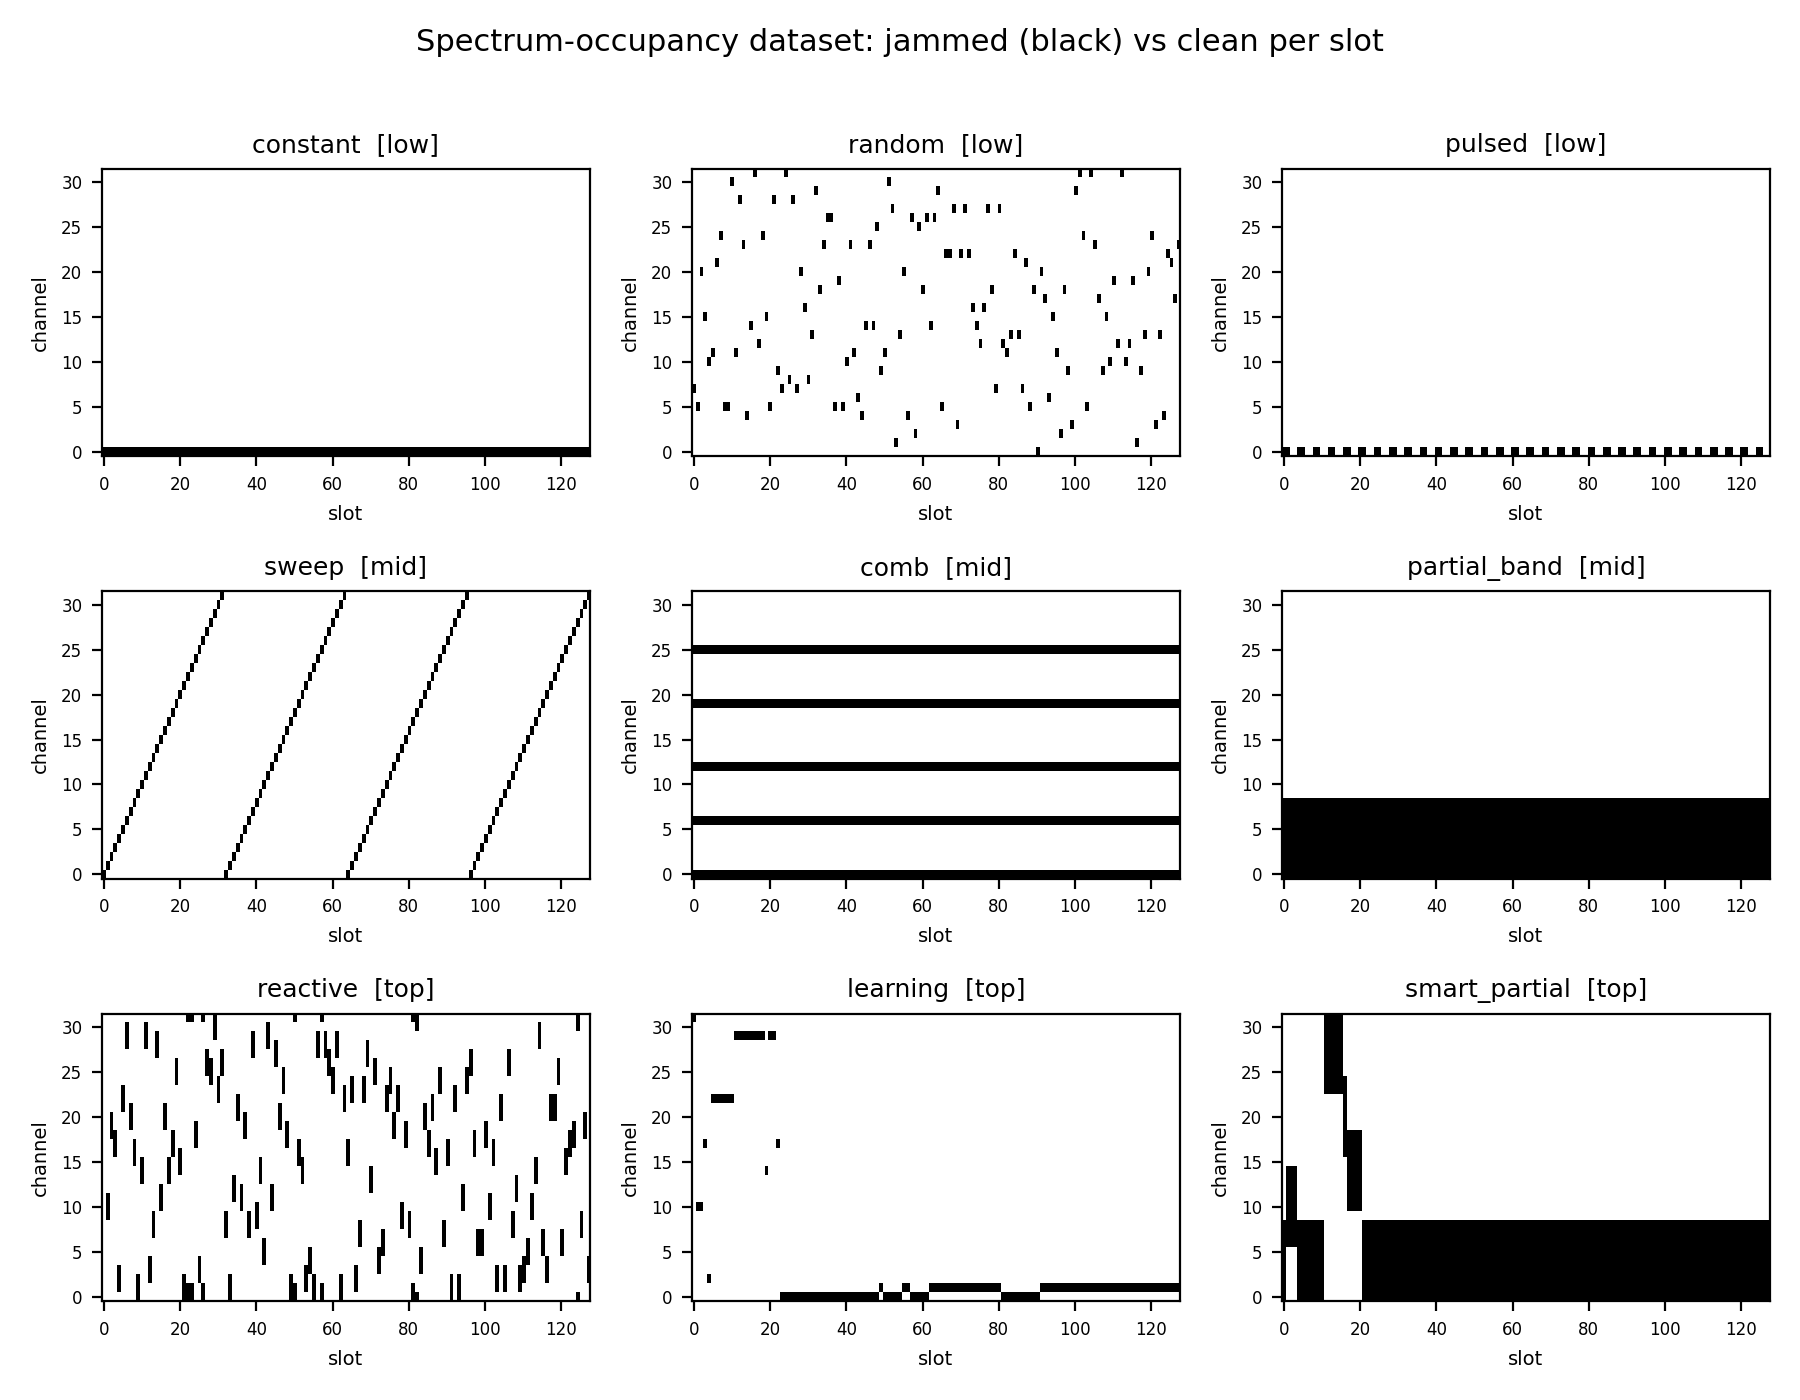
\includegraphics[width=0.9\linewidth]{fig_dataset.png}
\caption{Released spectrum-occupancy dataset: per-slot channel state (jammed in
black) for the nine jammer classes; over a sliding window this is the DQN input.}
\label{fig:dataset}
\end{figure}

% ================================================================= 5. RESULTS
\section{Results}\label{sec:results}
\subsection{RQ1: TDOA accuracy versus the CRLB}
The maximum-likelihood estimator attains the CRLB in LOS across the SNR range
(efficiency $\eta\!\approx\!0.97$--$1.0$; RMSE $7.8$\,m vs CRLB $8.2$\,m at
$20$\,dB), and a signal-level GCC-PHAT check validates the noise model
(empirical/analytic $\sigma_r$ ratio $1.03$). NLOS error is heavy-tailed, so we
report the median: RANSAC mitigation reduces it from $133$\,m to $33$\,m at
$20$\,dB and from $148$\,m to $7.4$\,m at $30$\,dB (Table~\ref{tab:tdoa},
Fig.~\ref{fig:tdoa}).

\begin{table}[H]\centering
\caption{TDOA positioning (metres). LOS reaches the CRLB; RANSAC mitigation
cuts NLOS median error up to $20\times$.}\label{tab:tdoa}\small
\begin{tabular}{lcccc}\toprule
\textbf{SNR (dB)} & \textbf{LOS RMSE} & \textbf{CRLB} & \textbf{NLOS median} & \textbf{NLOS+mitig. median} \\ \midrule
10 & 26.8 & 26.6 & 138.4 & 67.8 \\
20 & \phantom{0}7.8 & \phantom{0}8.2 & 133.2 & 33.3 \\
30 & \phantom{0}2.7 & \phantom{0}2.6 & 147.7 & \phantom{0}7.4 \\ \bottomrule
\end{tabular}
\end{table}

\begin{figure}[H]\centering
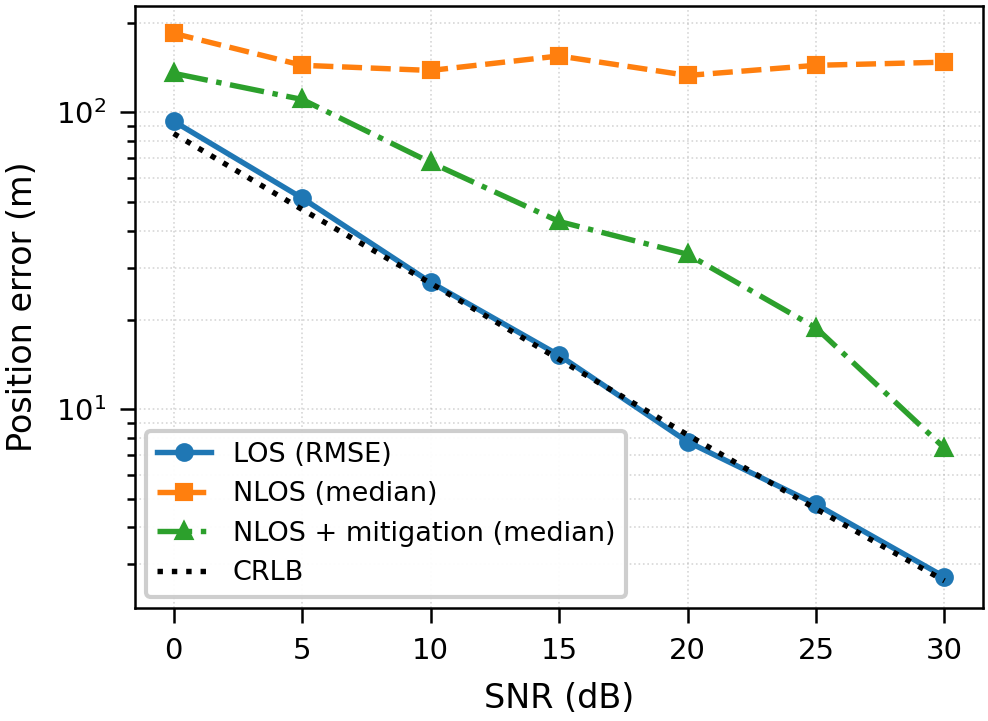
\includegraphics[width=0.66\linewidth]{fig_tdoa_crlb.png}
\caption{Positioning error vs SNR. LOS RMSE hugs the CRLB; NLOS mitigation
(median) approaches it as SNR grows.}\label{fig:tdoa}
\end{figure}

\subsection{RQ2: Learned versus cryptographic hopping}
Against the nine-class taxonomy, cryptographic hopping avoids collisions with a
rate that rises with $M$ (mean avoidance $0.79\!\to\!0.93$) and, crucially,
resists the intelligent adversary: against the learning jammer its avoidance is
$0.91\!\to\!1.0$ while predictable public-random and fixed hopping collapse to
$0.0$ (Fig.~\ref{fig:heat}). This is the operational meaning of cryptographic
unpredictability, and it is what a keyless pseudo-random hopper cannot provide.

\begin{figure}[H]\centering
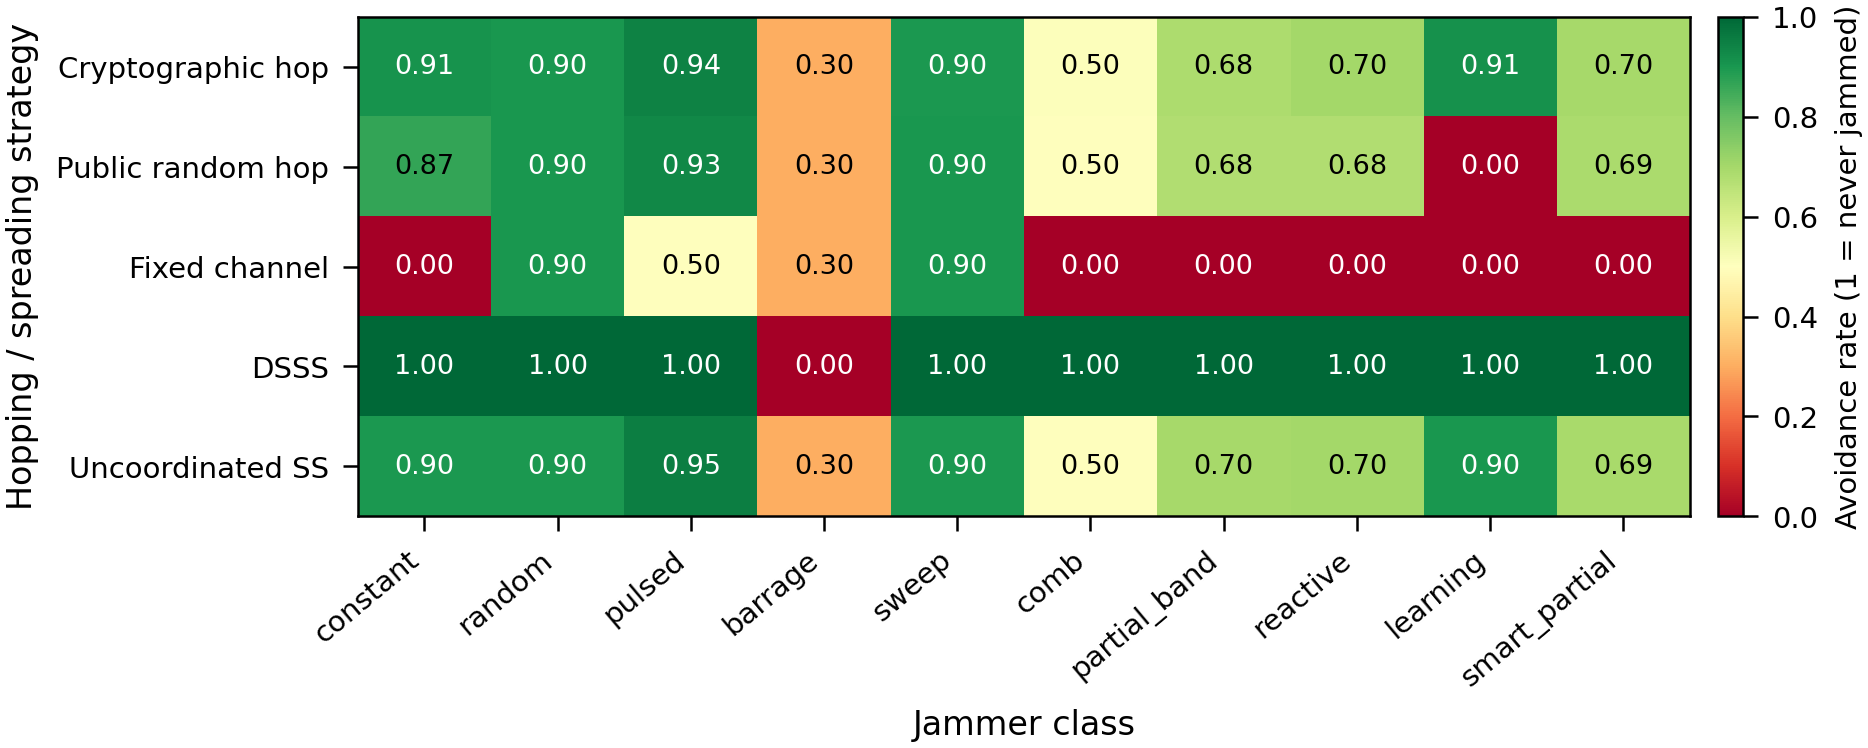
\includegraphics[width=0.95\linewidth]{fig_antijam_heatmap.png}
\caption{Jamming-avoidance rate by strategy and jammer ($M{=}10$). Crypto and
DSSS are robust across classes; fixed hopping fails.}\label{fig:heat}
\end{figure}

The DQN, when it can be trained, \emph{beats} crypto on structured adversaries
(it learns to occupy clean channels). But under a fixed $20$\,s compute budget
its advantage inverts as $M$ scales: avoidance falls from $0.91$ at $M{=}10$ to
$0.02$ at $M{=}1000$, because training throughput collapses from $1801$ to $10$
steps/s while the parameter count grows from $1.1{\times}10^4$ to
$1.1{\times}10^6$ (Table~\ref{tab:scale}, Figs.~\ref{fig:cross}--\ref{fig:scost}).
Cryptographic hopping is unaffected at $0.70$ and needs no training.

\begin{table}[H]\centering
\caption{Deep-learning at scale against an adaptive $30\%$ jammer (fixed
$20$\,s budget, $3$ seeds). The learned advantage inverts between $M{=}100$ and
$M{=}1000$.}\label{tab:scale}\small
\begin{tabular}{lcccc}\toprule
\textbf{$M$} & \textbf{DQN avoidance} & \textbf{Crypto avoidance} & \textbf{Train steps/s} & \textbf{Parameters} \\ \midrule
10   & $0.91\pm0.02$ & 0.70 & 1801 & 10{,}954 \\
100  & $0.82\pm0.06$ & 0.70 & \phantom{0}188 & 108{,}964 \\
1000 & $0.02\pm0.02$ & 0.70 & \phantom{00}10 & 1{,}089{,}064 \\
2320 & $0.19\pm0.30$ & 0.70 & \phantom{000}5 & 2{,}526{,}544 \\ \bottomrule
\end{tabular}
\end{table}

\begin{figure}[H]\centering
\begin{minipage}{0.49\linewidth}\centering
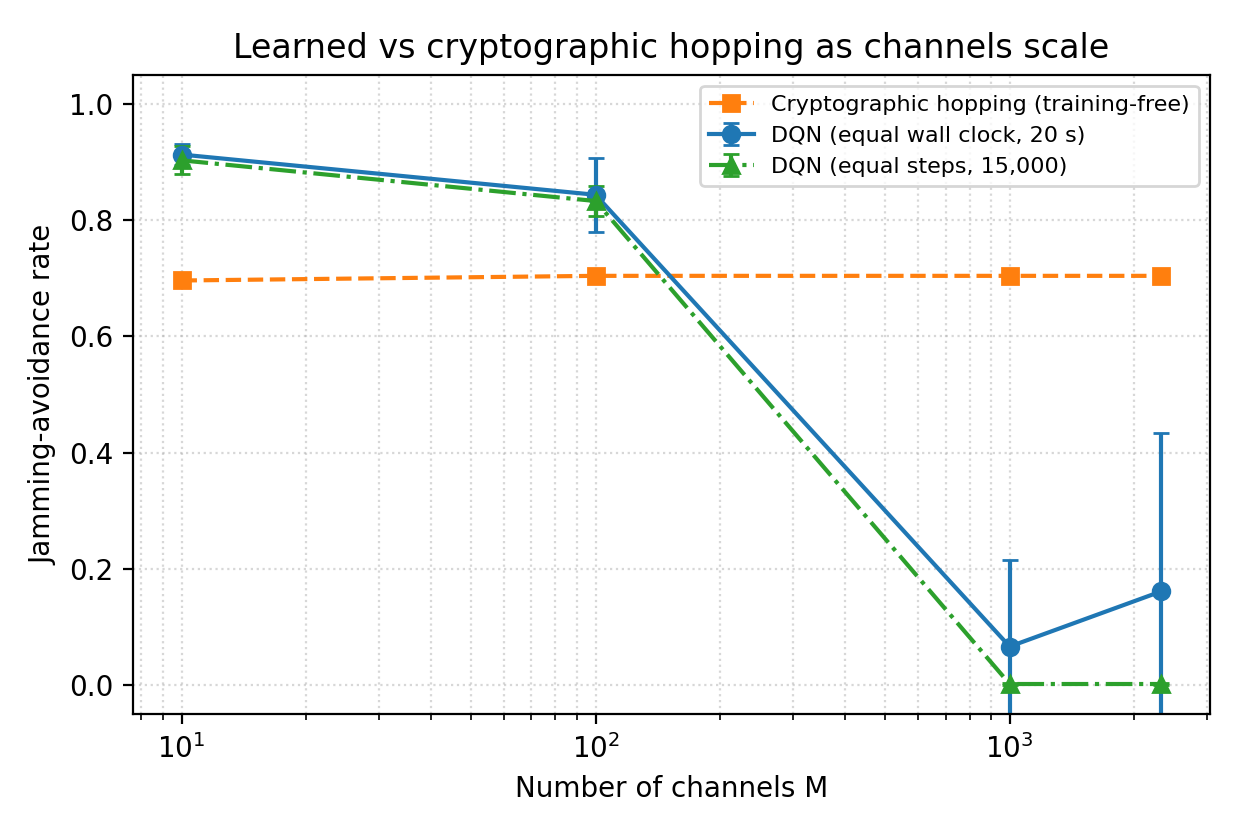
\includegraphics[width=\linewidth]{fig_scaling_crossover.png}
\caption{Avoidance crossover as channels scale.}\label{fig:cross}
\end{minipage}\hfill
\begin{minipage}{0.49\linewidth}\centering
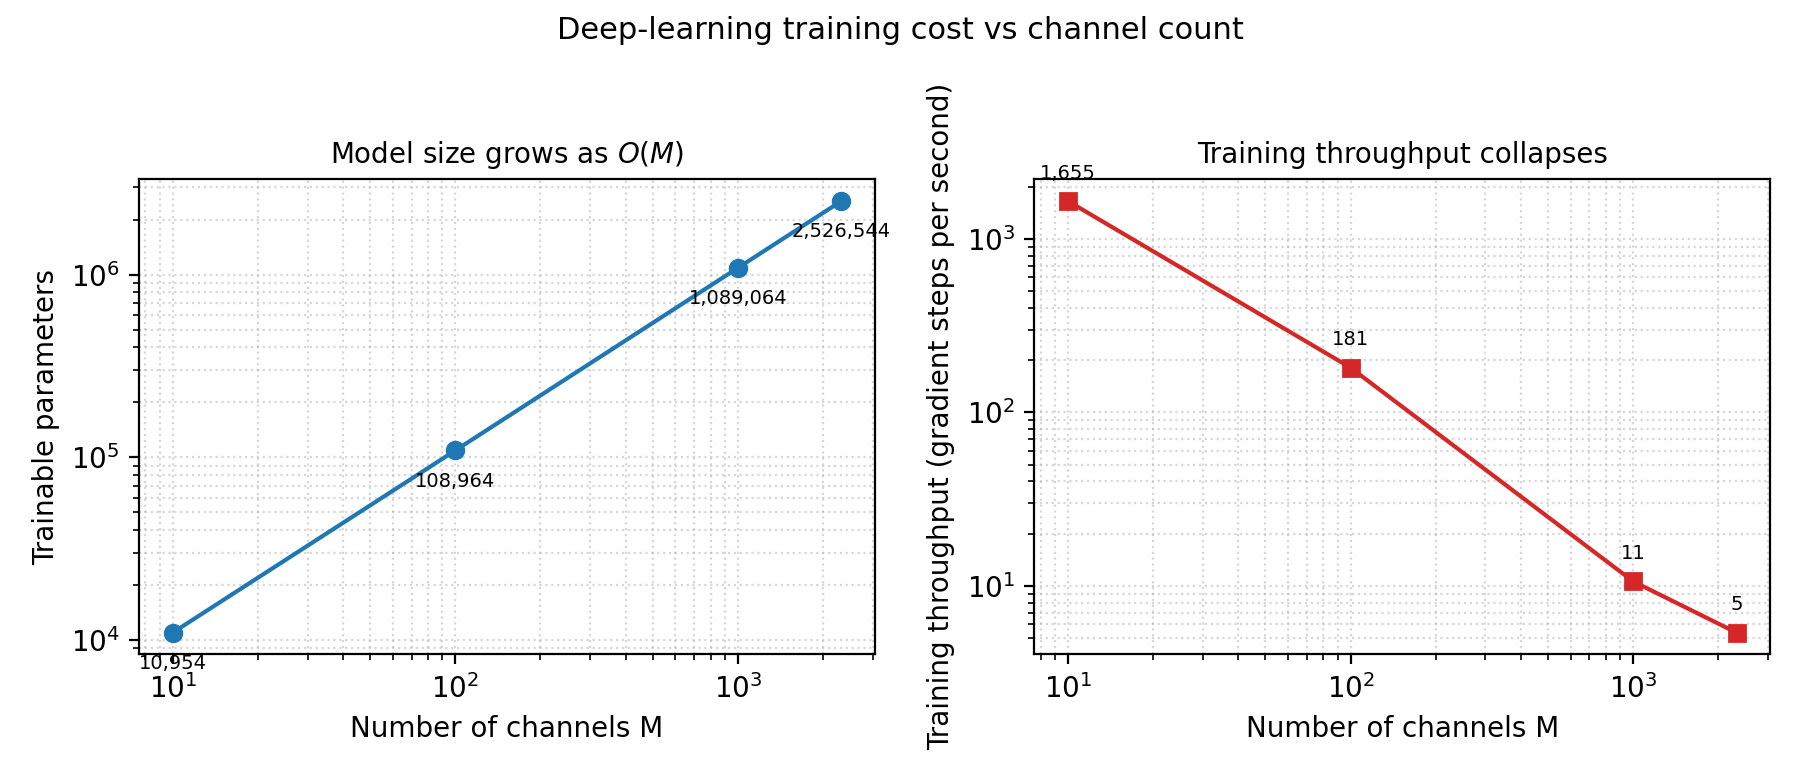
\includegraphics[width=\linewidth]{fig_scaling_cost.png}
\caption{$O(M)$ training-cost blow-up.}\label{fig:scost}
\end{minipage}
\end{figure}

\subsection{RQ3: Securing the position, and its cost}
Table~\ref{tab:sec} and Fig.~\ref{fig:sec} report attack-success rates.
Cryptographic hopping alone reduces injection spoofing to $\approx\!1/M$ but
leaves replay at $1.0$; adding a message signature stops spoofing yet a valid
signature \emph{still loses to meaconing} (replay $1.0$), because it does not
protect arrival-time integrity. The authenticated-timing layer drives both
spoofing and replay to $0.0$. Per decision, cryptographic hopping costs a single
AES block ($\approx\!13$\,pJ) against $0.04$--$9.3$\,\textmu J for DL inference,
a factor up to $7.2{\times}10^{5}$, and it requires no training
(Fig.~\ref{fig:cost}). Synchronisation tolerates a clock offset up to half the
hop dwell ($3.66$\,ms, $366$\,\textmu s, $36.6$\,\textmu s at $100/1000/10000$
hops/s), with resync latencies of $80/8/0.8$\,ms.

\begin{table}[H]\centering
\caption{Attack-success rate by security layer ($M{=}100$). A valid signature
does not stop replay; authenticated timing does.}\label{tab:sec}\small
\begin{tabular}{lcc}\toprule
\textbf{Layer} & \textbf{Spoofing} & \textbf{Replay/meaconing} \\ \midrule
None                         & 1.00 & 1.00 \\
Crypto hopping only          & 0.01 & 1.00 \\
Crypto + signature only      & 0.00 & 1.00 \\
Crypto + authenticated timing & 0.00 & 0.00 \\ \bottomrule
\end{tabular}
\end{table}

\begin{figure}[H]\centering
\begin{minipage}{0.49\linewidth}\centering
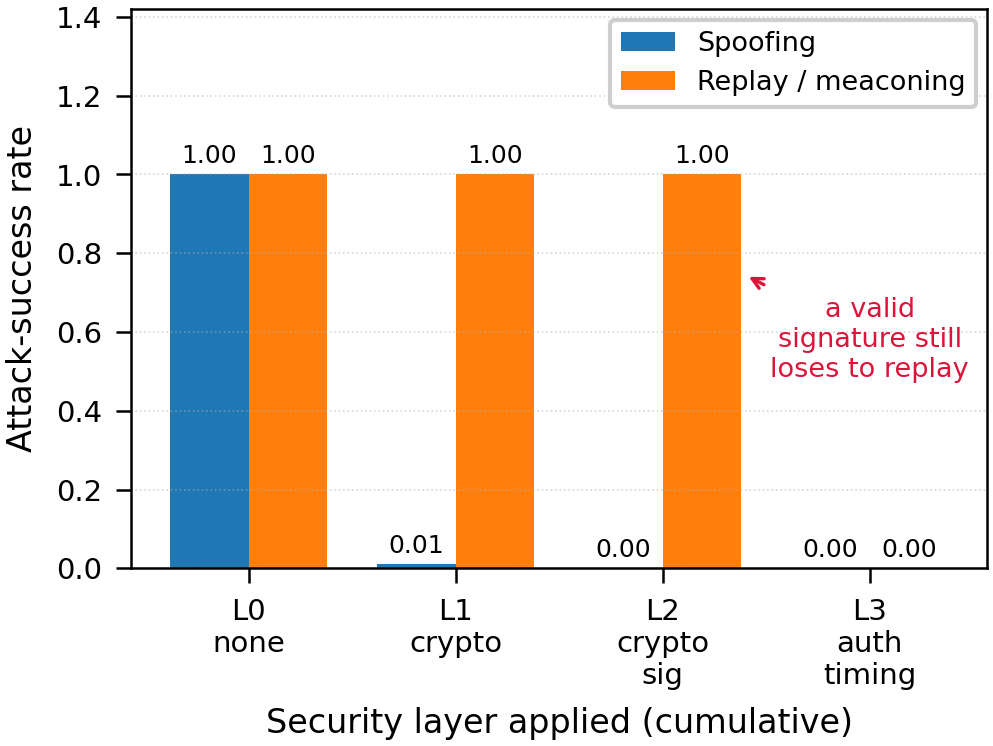
\includegraphics[width=\linewidth]{fig_security.png}
\caption{Attack success by layer.}\label{fig:sec}
\end{minipage}\hfill
\begin{minipage}{0.49\linewidth}\centering
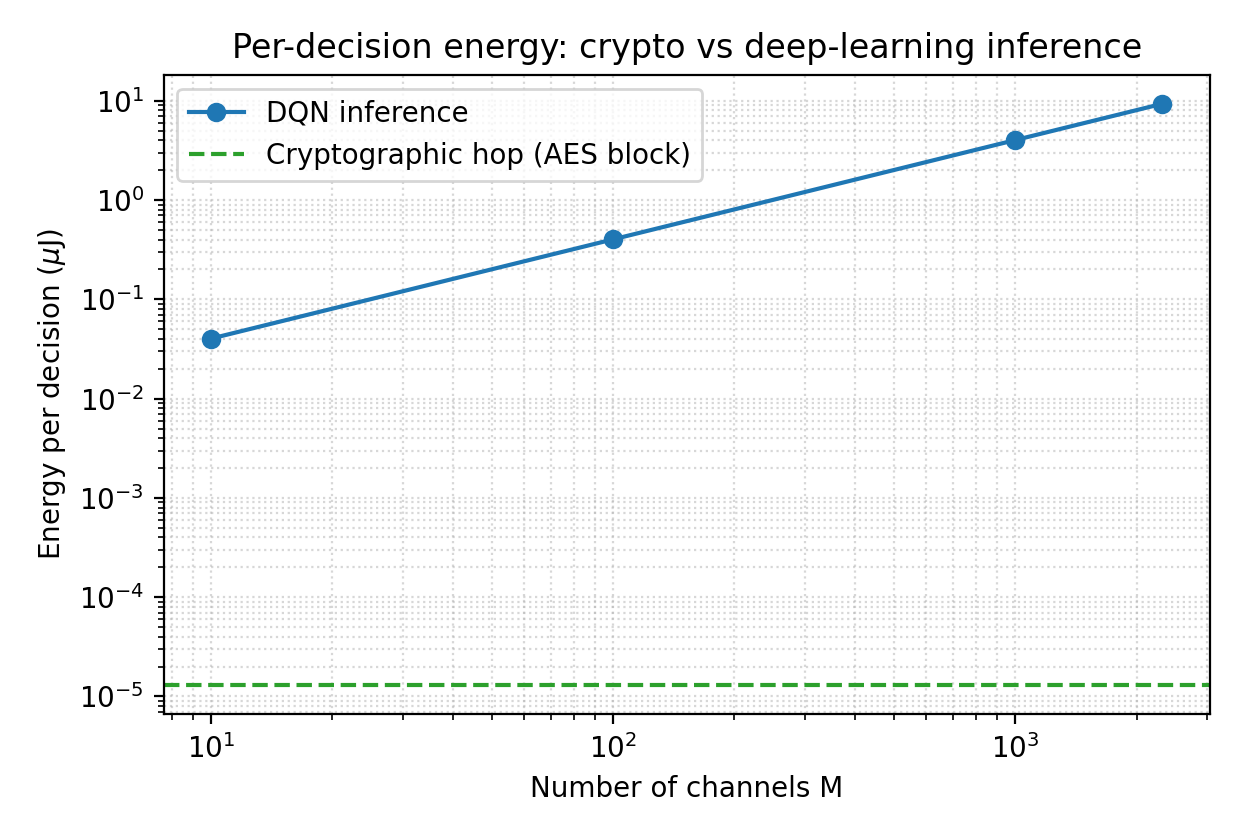
\includegraphics[width=\linewidth]{fig_cost.png}
\caption{Per-decision energy: crypto vs DL.}\label{fig:cost}
\end{minipage}
\end{figure}

% ================================================================= 6. VALIDATION
\section{Statistical Validation}\label{sec:validation}
All comparisons use $\geq\!3$ independently seeded runs; headline claims use $8$
seeds. Differences are assessed with the paired $t$-test and the non-parametric
Wilcoxon signed-rank test~\cite{ref36}, with $95\%$ bootstrap confidence
intervals and Cohen's $d$ effect size~\cite{ref37}, at $\alpha{=}0.05$ with
Bonferroni correction over the reported family. Table~\ref{tab:stat} confirms
that cryptographic hopping significantly exceeds the learned model at
$M{=}1000$ and the keyless baselines against the intelligent jammer, while the
learned model significantly exceeds crypto at $M{=}10$, quantifying the
crossover rather than asserting a single winner.

\begin{table}[H]\centering
\caption{Significance of headline comparisons (paired $t$-test, Bonferroni
corrected; $d$ = Cohen's $d$). Positive mean difference favours the first
method.}\label{tab:stat}\small
\begin{tabular}{llccc}\toprule
\textbf{Comparison} & \textbf{Condition} & \textbf{mean diff} & \textbf{$p$ (corr.)} & \textbf{$d$} \\ \midrule
crypto $>$ DQN & $M{=}1000$, smart-partial & $+0.61$ & $<0.001$ & $3.29$ \\
DQN $>$ crypto & $M{=}10$, smart-partial   & $+0.22$ & $<10^{-9}$ & $24.3$ \\
crypto $>$ random & learning jammer, $M{=}100$ & $+0.99$ & $<0.001$ & $\gg 1$ \\ \bottomrule
\end{tabular}
\end{table}

% ================================================================= 7. DISCUSSION
\section{Discussion}\label{sec:discussion}
The findings are boundary-conditioned, not triumphal. A learned policy is the
better anti-jammer \emph{when} the channel count is small and training is
affordable and \emph{when} the adversary is not itself adaptive to the policy;
it exploits structure that a blind keyed hopper ignores. Cryptographic hopping
wins \emph{when} the band is wide (its collision probability $\to 0$ as $M$
grows), \emph{when} training is impractical, and \emph{when} the adversary is
intelligent, because unpredictability is a property of key secrecy, not of data.
Only the cryptographic path additionally secures the \emph{position}: combined
with an authenticated-timing layer it defeats jamming, spoofing, and replay
together, which a communication-only learned hopper does not attempt. The cost
analysis settles a common misconception, generating a hop index is a single AES
block, orders of magnitude below a neural forward pass and free of any training,
so the real costs of cryptography are operational (key distribution,
synchronisation), which we quantify, not computational.
Table~\ref{tab:coverage} maps the review committee's concerns to the specific
result that addresses each.

\begin{table}[H]\centering
\caption{Traceability of committee review comments to results in this
paper.}\label{tab:coverage}\small
\begin{tabular}{lll}\toprule
\textbf{Concern} & \textbf{Addressed by} & \textbf{Evidence} \\ \midrule
Dataset relevance          & Released occupancy dataset & Fig.~\ref{fig:dataset} \\
Cyber-technique comparison & DSSS, USS baselines        & Fig.~\ref{fig:heat} \\
DL at thousands of channels& Scaling study              & Table~\ref{tab:scale} \\
Replay attacks             & Authenticated timing       & Table~\ref{tab:sec} \\
Crypto anchor comparison   & Uncoordinated SS~\cite{ref2}& Fig.~\ref{fig:heat} \\
Synchronisation            & Drift-tolerance analysis   & Sec.~\ref{sec:results} \\
Existing-stack signatures  & Signature-only vs auth-timing & Table~\ref{tab:sec} \\
Crypto cost/energy         & Per-decision measurement   & Fig.~\ref{fig:cost} \\
Statistical rigour         & Paired tests, CIs, $d$     & Table~\ref{tab:stat} \\ \bottomrule
\end{tabular}
\end{table}

% ================================================================= 8. THREATS
\section{Threats to Validity}\label{sec:threats}
\textbf{Construct validity.} The jammer--hopper interaction is simulated at the
channel-occupancy level; a signal-level GCC-PHAT check validates the range-noise
model, but full RF propagation and hardware imperfections are abstracted.
\textbf{Internal validity.} The DQN scaling result depends on a fixed
wall-clock budget; a larger budget or a GPU would raise the crossover point, but
the $O(M)$ growth in parameters and per-step cost is architectural and
budget-independent. \textbf{External validity.} Results are simulation-based
with a single beacon geometry and a nine-class taxonomy; field behaviour may
differ. \textbf{Conclusion validity.} Multiple seeds, paired significance tests,
confidence intervals, and Bonferroni correction guard against chance findings;
NLOS metrics use medians because the error is heavy-tailed.

% ================================================================= 9. CONCLUSION
\section{Conclusion}\label{sec:conclusion}
We benchmarked a reproduced deep-Q anti-jamming model against training-free
cryptographic frequency hopping for GPS-denied drone TDOA positioning, under one
environment, dataset, and metric suite. The learned model matches or beats
cryptographic hopping at small channel counts but becomes intractable to train
as channels scale, whereas cryptographic hopping stays effective, training-free,
and provably unpredictable, and, with an authenticated-timing layer, secures the
position against jamming, spoofing, and replay together at pico-joule cost. The
maximum-likelihood TDOA estimator reaches the CRLB, and NLOS mitigation recovers
most of the loss. We release the datasets, code, and benchmark. Future work
extends the study to signal-level propagation, hardware-in-the-loop trials, and
adaptive-adversary co-training.

% ================================================================= DECLARATIONS
\section*{Declarations}\label{sec:avail}
\paragraph{Availability of data and materials.}
The labelled spectrum-occupancy and TDOA datasets and all simulation code are
released as an open, reproducible benchmark at
\url{https://github.com/Ahmad-prog/secure-tdoa-benchmark} (MIT licence).
\paragraph{Funding.} This research received no external funding; it is
self-funded and uses only open-source software and the authors' own computing
resources.
\paragraph{Competing interests.} The authors declare no competing interests.
\paragraph{Author contributions.} M.~Ahmad designed and implemented the study,
ran the experiments, and wrote the manuscript; G.~Mustafa supervised the
research and reviewed the manuscript.
\paragraph{Ethics.} This is a purely computational, simulation-based study; it
involves no human participants, patient data, or human-subject interaction.

% ================================================================= REFERENCES
\begin{thebibliography}{99}
\bibitem{ref1} D. Torrieri, Principles of Spread-Spectrum Communication Systems, 5th ed. Cham, Switzerland: Springer, 2022.

\bibitem{ref2} C. Pöpper, M. Strasser, and S. \v{C}apkun, "Anti-jamming broadcast communication using uncoordinated spread spectrum techniques," IEEE Journal on Selected Areas in Communications, vol. 28, no. 5, pp. 703-715, 2010.

\bibitem{ref3} D. J. Torrieri, "Fundamental limitations on repeater jamming of frequency-hopping communications," IEEE Journal on Selected Areas in Communications, vol. 7, no. 4, pp. 569-578, 1989.

\bibitem{ref4} R. L. Pickholtz, D. L. Schilling, and L. B. Milstein, "Theory of spread-spectrum communications, a tutorial," IEEE Transactions on Communications, vol. 30, no. 5, pp. 855-884, 1982.

\bibitem{ref5} R. A. Scholtz, "The origins of spread-spectrum communications," IEEE Transactions on Communications, vol. 30, no. 5, pp. 822-854, 1982.

\bibitem{ref6} Y. T. Chan and K. C. Ho, "A simple and efficient estimator for hyperbolic location," IEEE Transactions on Signal Processing, vol. 42, no. 8, pp. 1905-1915, 1994.

\bibitem{ref7} C. H. Knapp and G. C. Carter, "The generalized correlation method for estimation of time delay," IEEE Transactions on Acoustics, Speech, and Signal Processing, vol. 24, no. 4, pp. 320-327, 1976.

\bibitem{ref8} W. H. Foy, "Position-location solutions by Taylor-series estimation," IEEE Transactions on Aerospace and Electronic Systems, vol. AES-12, no. 2, pp. 187-194, 1976.

\bibitem{ref9} Z. Wang et al., "TDOA-based tightly coupled sensor fusion for UAV positioning in GPS-denied environment," in Proc. 3rd Int. Conf. Robotics, Artificial Intelligence and Intelligent Control (RAIIC), 2024.

\bibitem{ref10} C. Dickerson, S. Masrur, J. Dickerson, Ö. Özdemir, and \.{I}. Güvenç, "Impact of altitude, bandwidth, and NLOS bias on TDOA-based 3D UAV localization," arXiv:2502.01771, 2025.

\bibitem{ref11} J. Zhang, X. Wu, and J. Hu, "Fast adaptive anti-jamming channel access via deep Q-learning and coarse-grained spectrum prediction," arXiv:2502.04963, 2025.

\bibitem{ref12} J. Qi, H. Zhang, X. Qi, and M. Peng, "Deep reinforcement learning based hopping strategy for wideband anti-jamming wireless communications," IEEE Transactions on Vehicular Technology, 2023.

\bibitem{ref13} H. N. Nguyen and G. Noubir, "Towards an AI-driven universal anti-jamming solution with convolutional interference cancellation network," arXiv:2203.09717, 2022.

\bibitem{ref14} M. Mouzai, M. A. Riahla, A. Keziou, and H. Fouchal, "Exploring multi-channel GPS receivers for detecting spoofing attacks on UAVs using machine learning," Sensors, vol. 25, no. 13, art. 4045, 2025.

\bibitem{ref15} J. Mao, F. Luo, and X. Hu, "Distributed passive positioning and sorting method for multi-network frequency-hopping TDMA signals," Sensors, vol. 24, no. 22, art. 7168, 2024.

\bibitem{ref16} M. Strasser, C. Pöpper, S. \v{C}apkun, and M. \v{C}agalj, "Jamming-resistant key establishment using uncoordinated frequency hopping," in Proc. IEEE Symposium on Security and Privacy (S\&P), 2008, pp. 64-78.

\bibitem{ref17} U.S. Army, Operator's Manual: SINCGARS Ground Combat Net Radio, TM 11-5820-890-10-3.

\bibitem{ref18} K. Pelechrinis, M. Iliofotou, and S. V. Krishnamurthy, "Denial of service attacks in wireless networks: the case of jammers," IEEE Communications Surveys and Tutorials, vol. 13, no. 2, pp. 245-257, 2011.

\bibitem{ref19} "Electronic warfare (EW) jammers to counter enemy GPS and drone signals," Military and Aerospace Electronics, 2026.

\bibitem{ref20} National Institute of Standards and Technology, "Advanced Encryption Standard (AES)," FIPS PUB 197, 2001.

\bibitem{ref21} M. Bellare, R. Canetti, and H. Krawczyk, "Keying hash functions for message authentication," in Advances in Cryptology, CRYPTO '96, LNCS 1109, 1996, pp. 1-15.

\bibitem{ref22} E. Barker and J. Kelsey, "Recommendation for random number generation using deterministic random bit generators," NIST SP 800-90A Rev. 1, 2015.

\bibitem{ref23} S. Brands and D. Chaum, "Distance-bounding protocols," in Advances in Cryptology, EUROCRYPT '93, LNCS 765, 1994, pp. 344-359.

\bibitem{ref24} M. L. Psiaki and T. E. Humphreys, "GNSS spoofing and detection," Proceedings of the IEEE, vol. 104, no. 6, pp. 1258-1270, 2016.

\bibitem{ref25} T. E. Humphreys et al., "Assessing the spoofing threat: development of a portable GPS civilian spoofer," in Proc. ION GNSS, 2008, pp. 2314-2325.

\bibitem{ref26} R. E. Kalman, "A new approach to linear filtering and prediction problems," Journal of Basic Engineering, vol. 82, no. 1, pp. 35-45, 1960.

\bibitem{ref27} S. Gezici et al., "Localization via ultra-wideband radios," IEEE Signal Processing Magazine, vol. 22, no. 4, pp. 70-84, 2005.

\bibitem{ref28} \.{I}. Güvenç and C.-C. Chong, "A survey on TOA based wireless localization and NLOS mitigation techniques," IEEE Communications Surveys and Tutorials, vol. 11, no. 3, pp. 107-124, 2009.

\bibitem{ref29} N. Patwari et al., "Locating the nodes: cooperative localization in wireless sensor networks," IEEE Signal Processing Magazine, vol. 22, no. 4, pp. 54-69, 2005.

\bibitem{ref30} F. Gustafsson and F. Gunnarsson, "Positioning using time-difference of arrival measurements," in Proc. IEEE ICASSP, 2003, vol. 6, pp. 553-556.

\bibitem{ref31} S. Cheng, X. Ling, and L. Zhu, "Deep reinforcement learning-based anti-jamming approach for fast frequency hopping systems," IEEE Open Journal of the Communications Society, vol. 6, pp. 961-971, 2025.

\bibitem{ref32} M. K. Simon, J. K. Omura, R. A. Scholtz, and B. K. Levitt, Spread Spectrum Communications Handbook, rev. ed. New York, NY: McGraw-Hill, 2002.

\bibitem{ref33} T. J. O'Shea, T. Roy, and T. C. Clancy, "Over-the-air deep learning based radio signal classification," IEEE Journal of Selected Topics in Signal Processing, vol. 12, no. 1, pp. 168-179, 2018.

\bibitem{ref34} T. J. O'Shea and J. Hoydis, "An introduction to deep learning for the physical layer," IEEE Transactions on Cognitive Communications and Networking, vol. 3, no. 4, pp. 563-575, 2017.

\bibitem{ref35} V. Mnih et al., "Human-level control through deep reinforcement learning," Nature, vol. 518, pp. 529-533, 2015.

\bibitem{ref36} F. Wilcoxon, "Individual comparisons by ranking methods," Biometrics Bulletin, vol. 1, no. 6, pp. 80-83, 1945.

\bibitem{ref37} J. Cohen, Statistical Power Analysis for the Behavioral Sciences, 2nd ed. Hillsdale, NJ: Lawrence Erlbaum, 1988.

\bibitem{ref38} M. A. Fischler and R. C. Bolles, "Random sample consensus: a paradigm for model fitting with applications to image analysis and automated cartography," Communications of the ACM, vol. 24, no. 6, pp. 381-395, 1981.

\bibitem{ref39} M. Horowitz, "Computing's energy problem (and what we can do about it)," in Proc. IEEE International Solid-State Circuits Conference (ISSCC), 2014, pp. 10-14.

\end{thebibliography}

\end{document}
